
\documentclass[11pt,a4paper]{article}
\usepackage[utf8]{inputenc}
\usepackage[T1]{fontenc}
\usepackage[spanish,es-nodecimaldot]{babel}
\usepackage{lmodern}
\usepackage{microtype}
\usepackage{geometry}
\usepackage{graphicx}
\usepackage{booktabs}
\usepackage{array}
\usepackage{tabularx}
\usepackage{adjustbox}
\usepackage{amsmath}
\usepackage{amssymb}
\usepackage{float}
\usepackage{subcaption}
\usepackage{xcolor}
\usepackage{hyperref}
\geometry{margin=2.2cm}
\usepackage{mathtools,bm}
\usepackage{microtype}



\definecolor{burgundy}{HTML}{7A1E2C}
\definecolor{charcoal}{HTML}{3A3A3A}
\hypersetup{colorlinks=true, linkcolor=burgundy, citecolor=burgundy, urlcolor=burgundy}
\setlength{\tabcolsep}{5pt}
\renewcommand{\arraystretch}{1.16}
\graphicspath{{figures/}}

\title{Clasificación de patrones chartistas en BRENT mediante ventanas multiactivo codificadas en RGB y EfficientNet-B1}
\author{}
\date{}

\begin{document}
\maketitle

\begin{abstract}
Este trabajo evalúa un pipeline de clasificación de patrones chartistas sobre BRENT construido a partir de un bundle multiactivo. El experimento utiliza series temporales de commodities, principales referencias en interest rates e indices de equity con mayor relevancia , una matriz \emph{wide} con 7004 filas temporales y 180 variables seleccionadas, y tensores precomputados de tamaño 32\,$\times$\,180. La representación de cada ventana se realiza mediante una codificación RGB compuesta por GASF del nivel de BRENT, GADF de su retorno reciente y un mapa multivariante de variables estandarizadas; sobre esa imagen se entrena un modelo multitarea con \emph{backbone} EfficientNet-B1. En la corrida analizada, con \emph{lookback} 32, horizonte de retorno de un día, tamaño de imagen 160\,$\times$\,160, CPU y un régimen corto de 1+1 épocas, la evaluación sobre el tramo de \emph{test} alcanza una exactitud del 53.3\% y una exactitud top-2 del 81.6\% frente a las etiquetas débiles del sistema. Para la regresión del retorno a un día del BRENT, la MAE es 2.64 puntos porcentuales y la RMSE 3.40 puntos porcentuales. La última señal disponible, fechada el 6 de marzo de 2026, asigna la clase \texttt{ascending\_channel} con probabilidad 0.842 y un retorno esperado de 0.987\%.
\end{abstract}

\section{Introducción}
La identificación automática de patrones chartistas sigue siendo un problema relevante cuando el objetivo no es únicamente anticipar el siguiente retorno, sino describir la geometría reciente del precio dentro de un contexto de mercado más amplio. En este estudio el activo objetivo es el BRENT, pero la entrada no se limita a su trayectoria aislada: el modelo observa simultáneamente divisas, materias primas, índices de renta variable y tipos de interés agregados en un bundle multiactivo. La propuesta conecta tres ideas: etiquetado débil de figuras técnicas \cite{lo2000foundations}, transformación de series temporales en imágenes mediante \emph{Gramian Angular Fields} \cite{wang2015imaging} y extracción de representaciones con EfficientNet-B1 \cite{tan2019efficientnet}.

El interés académico del experimento reside en dos niveles. Primero, permite estudiar si una representación visual compacta conserva información suficiente para discriminar estructuras chartistas sobre ventanas relativamente cortas. Segundo, ofrece una base cuantitativa para comparar clasificación de patrones y predicción de retorno dentro del mismo esquema multitarea.

\section{Datos e inputs del experimento}
El proceso parte de las series definidas en \texttt{SeriesDownloader\_2\_features.py}. El script solicita 28 series de Yahoo Finance, 9 series de FRED y 4 nodos de la curva AAA del BCE. Tras la construcción del bundle final, el experimento conserva 37 series base y 180 variables de entrada. La Tabla~\ref{tab:inputs} resume los inputs operativos del estudio, mientras que la Figura~\ref{fig:sources} sintetiza el universo solicitado por fuente.

\begin{table}[H]
\centering
\footnotesize
\caption{Inputs del experimento y configuración efectiva de la corrida analizada.}
\label{tab:inputs}
\begin{adjustbox}{max width=\textwidth}
\begin{tabular}{p{0.58\textwidth}p{0.26\textwidth}}
\toprule
                                      Input &              Valor \\
\midrule
Series solicitadas (Yahoo / FRED / BCE AAA) &         28 / 9 / 4 \\
   Series base presentes en el bundle final &                 37 \\
         Variables de entrada seleccionadas &                180 \\
               Variable objetivo del bundle & BRENT\_fwd\_logret\_1 \\
                            Activo objetivo &              BRENT \\
                Ventana temporal (lookback) &            32 días \\
                       Horizonte de retorno &              1 día \\
           Horizonte de soporte/resistencia &             5 días \\
                       Resolución de imagen &          160 x 160 \\
                         Split precomputado &                 Sí \\
   Validación dentro del train precomputado &                10\% \\
                                Dispositivo &                CPU \\
             Épocas (warm-up / fine-tuning) &              1 / 1 \\
\bottomrule
\end{tabular}

\end{adjustbox}
\end{table}

\begin{figure}[H]
    \centering
    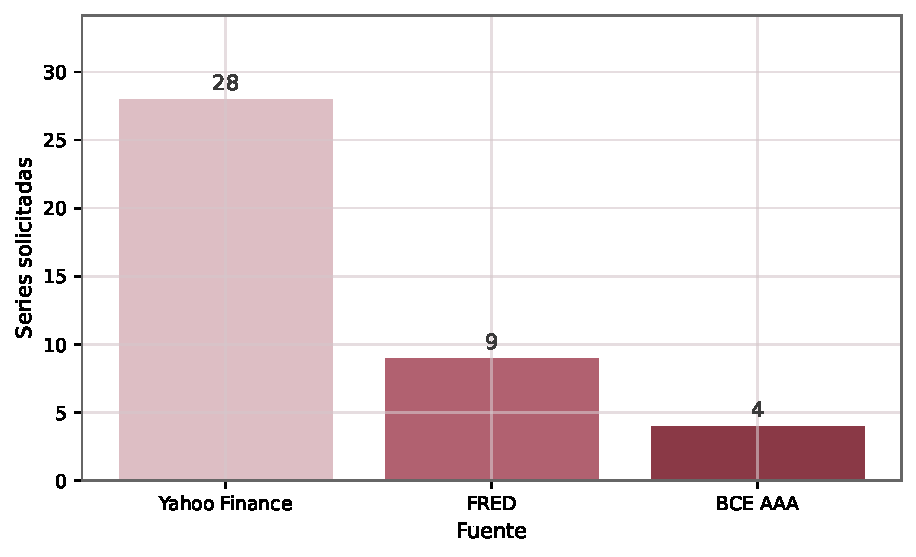
\includegraphics[width=0.60\textwidth]{source_counts.pdf}
    \caption{Número de series solicitadas por fuente en el descargador.}
    \label{fig:sources}
\end{figure}

Las variables del bundle se organizan en seis grupos: cierres, retornos logarítmicos a un día, volatilidad móvil a 20 días, rango intradiario relativo, relación de medias móviles 5/20 y spreads o ratios derivados. La Figura~\ref{fig:featuregroups} y la Tabla~\ref{tab:featuregroups} muestran esta descomposición.

\begin{figure}[H]
    \centering
    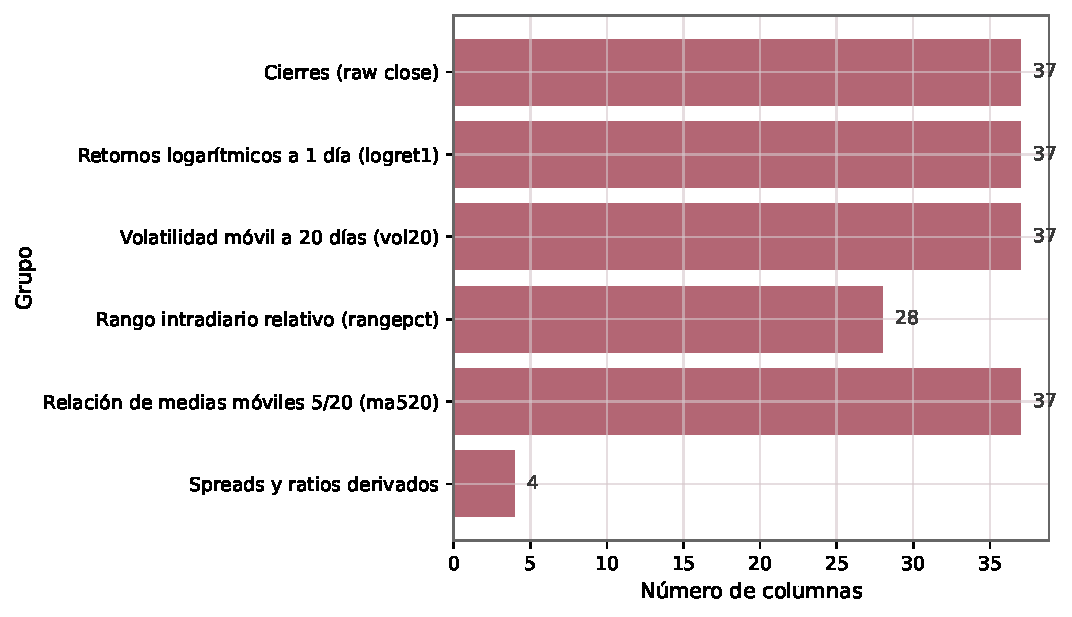
\includegraphics[width=0.72\textwidth]{feature_groups.pdf}
    \caption{Descomposición de las variables del bundle final.}
    \label{fig:featuregroups}
\end{figure}

\begin{table}[H]
\centering
\footnotesize
\caption{Grupos de variables utilizados en la representación multiactivo.}
\label{tab:featuregroups}
\begin{adjustbox}{max width=0.82\textwidth}
\begin{tabular}{p{0.58\textwidth}r}
\toprule
                     Grupo de variables &  Número \\
\midrule
                    Cierres (raw close) &      37 \\
Retornos logarítmicos a 1 día (logret1) &      37 \\
    Volatilidad móvil a 20 días (vol20) &      37 \\
  Rango intradiario relativo (rangepct) &      28 \\
Relación de medias móviles 5/20 (ma520) &      37 \\
             Spreads y ratios derivados &       4 \\
\bottomrule
\end{tabular}

\end{adjustbox}
\end{table}

La cobertura temporal efectiva no comienza al inicio histórico del precio, sino cuando todas las variables necesarias están simultáneamente disponibles. Las features más tardías están asociadas a \texttt{ESTR} y \texttt{SOFR}, lo que desplaza el arranque de las ventanas plenamente válidas a finales de 2019. La Figura~\ref{fig:latestfeatures} recoge las variables que más condicionan ese punto de inicio.

\begin{figure}[H]
    \centering
    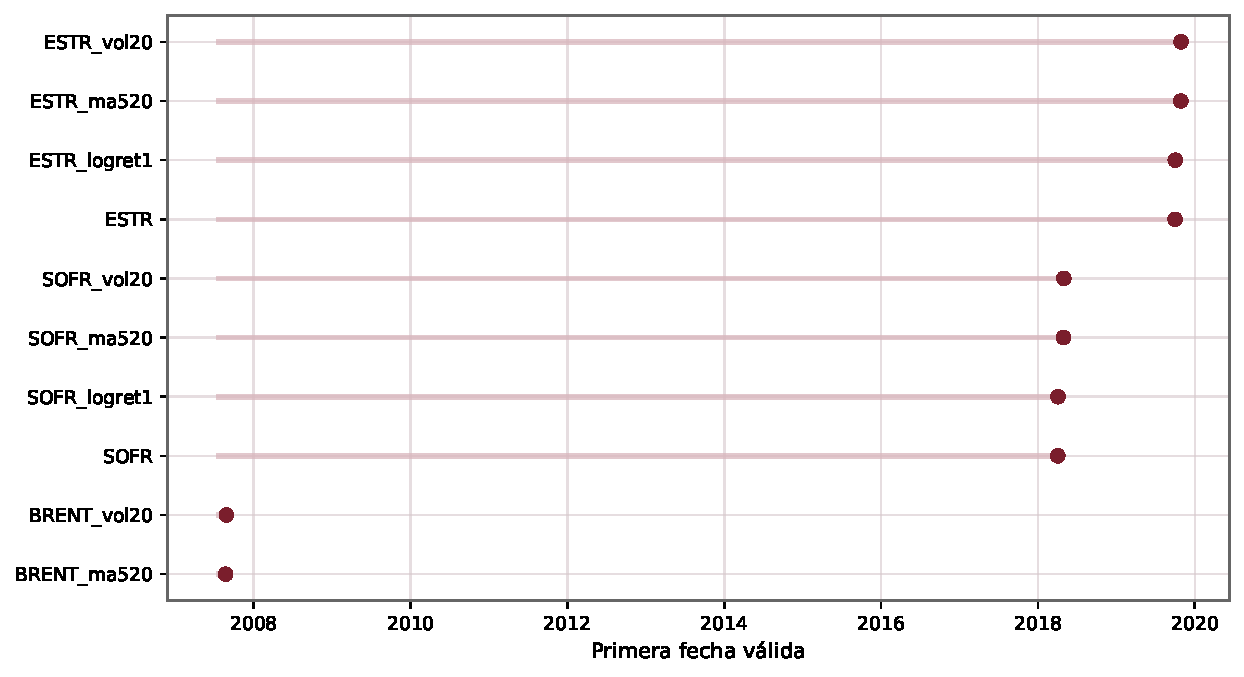
\includegraphics[width=0.84\textwidth]{latest_starting_features.pdf}
    \caption{Variables con fecha de primera observación válida más tardía dentro del bundle.}
    \label{fig:latestfeatures}
\end{figure}

El script solicita además los nodos \texttt{EUR\_AAA\_2Y}, \texttt{EUR\_AAA\_5Y}, \texttt{EUR\_AAA\_10Y} y \texttt{EUR\_AAA\_30Y}; sin embargo, dichas series no aparecen en el bundle final suministrado. Por tanto, la versión empírica aquí evaluada se apoya en el conjunto de 37 series efectivamente presentes.

\subsection{Ventana temporal y particiones}
La representación se construye sobre ventanas de 32 observaciones y el target principal es el retorno futuro a un día, \texttt{BRENT\_fwd\_logret\_1}. Los tensores precomputados aportan 986 ventanas para train y 247 para test. Sobre el bloque de train se reserva un 10\% para validación interna. La evaluación completa con etiquetas débiles y salidas continuas utiliza 1230 ventanas: 887 en train, 99 en validación y 244 en test. Las tres últimas ventanas del tensor de test quedan fuera de esa evaluación porque no disponen del horizonte completo de cinco días empleado para \texttt{future\_low} y \texttt{future\_high}. La Tabla~\ref{tab:splits} resume las particiones temporales.

\begin{table}[H]
\centering
\footnotesize
\caption{Particiones temporales del experimento.}
\label{tab:splits}
\begin{adjustbox}{max width=\textwidth}
\begin{tabular}{p{0.24\textwidth}rllp{0.28\textwidth}}
\toprule
                 Partición &  Ventanas &     Inicio &        Fin &                                Uso \\
\midrule
Tensor precomputado: train &       986 & 2019-12-02 & 2024-11-20 & Entrenamiento + validación interna \\
 Tensor precomputado: test &       247 & 2024-11-21 & 2026-03-04 &                  Hold-out temporal \\
          Train etiquetado &       887 & 2019-12-02 & 2024-05-21 &                             Ajuste \\
     Validación etiquetada &        99 & 2024-05-22 & 2024-11-20 &                  Selección interna \\
           Test etiquetado &       244 & 2024-11-21 & 2026-02-26 &                   Evaluación final \\
\bottomrule
\end{tabular}

\end{adjustbox}
\end{table}

\section{Metodología}
\subsection{Etiquetado débil y objetivo supervisado}
El sistema asigna a cada ventana una etiqueta débil de patrón chartista a partir de reglas geométricas y de estructura local sobre el precio del BRENT. Las clases contempladas son \texttt{double\_bottom}, \texttt{double\_top}, \texttt{ascending\_channel}, \texttt{descending\_channel}, \texttt{high\_tight\_flag}, \texttt{head\_shoulders}, \texttt{inverse\_head\_shoulders} y \texttt{range}. Una ventana recibe la clase de máxima puntuación cuando la confianza supera el umbral mínimo configurado, fijado en 0.35 para esta corrida.

Además de la clasificación, el modelo estima tres salidas continuas: retorno futuro, mínimo relativo futuro y máximo relativo futuro. Esto permite evaluar conjuntamente la capacidad de reconocimiento de patrón y la utilidad direccional de la representación temporal.

\subsection{Representación RGB de la ventana}
Cada muestra utiliza una ventana de 32 pasos y 180 variables. La imagen RGB se construye con tres canales: \emph{Gramian Angular Summation Field} (GASF) del nivel de BRENT, \emph{Gramian Angular Difference Field} (GADF) de su retorno reciente y un mapa multivariante derivado de las variables estandarizadas del bundle. Si $x_t$ es una serie reescalada a $[-1,1]$ y $\phi_t = \arccos(x_t)$, entonces:
\begin{equation}
\mathrm{GASF}_{ij} = \cos(\phi_i + \phi_j),
\end{equation}
\begin{equation}
\mathrm{GADF}_{ij} = \sin(\phi_i - \phi_j).
\end{equation}

La Figura~\ref{fig:rgbexample} muestra un ejemplo real de codificación para una ventana del tramo final de test, y la Figura~\ref{fig:examplewindow} ilustra la relación entre la ventana de entrada y el corredor futuro de cinco días usado en las variables \texttt{future\_low} y \texttt{future\_high}.

\begin{figure}[H]
    \centering
    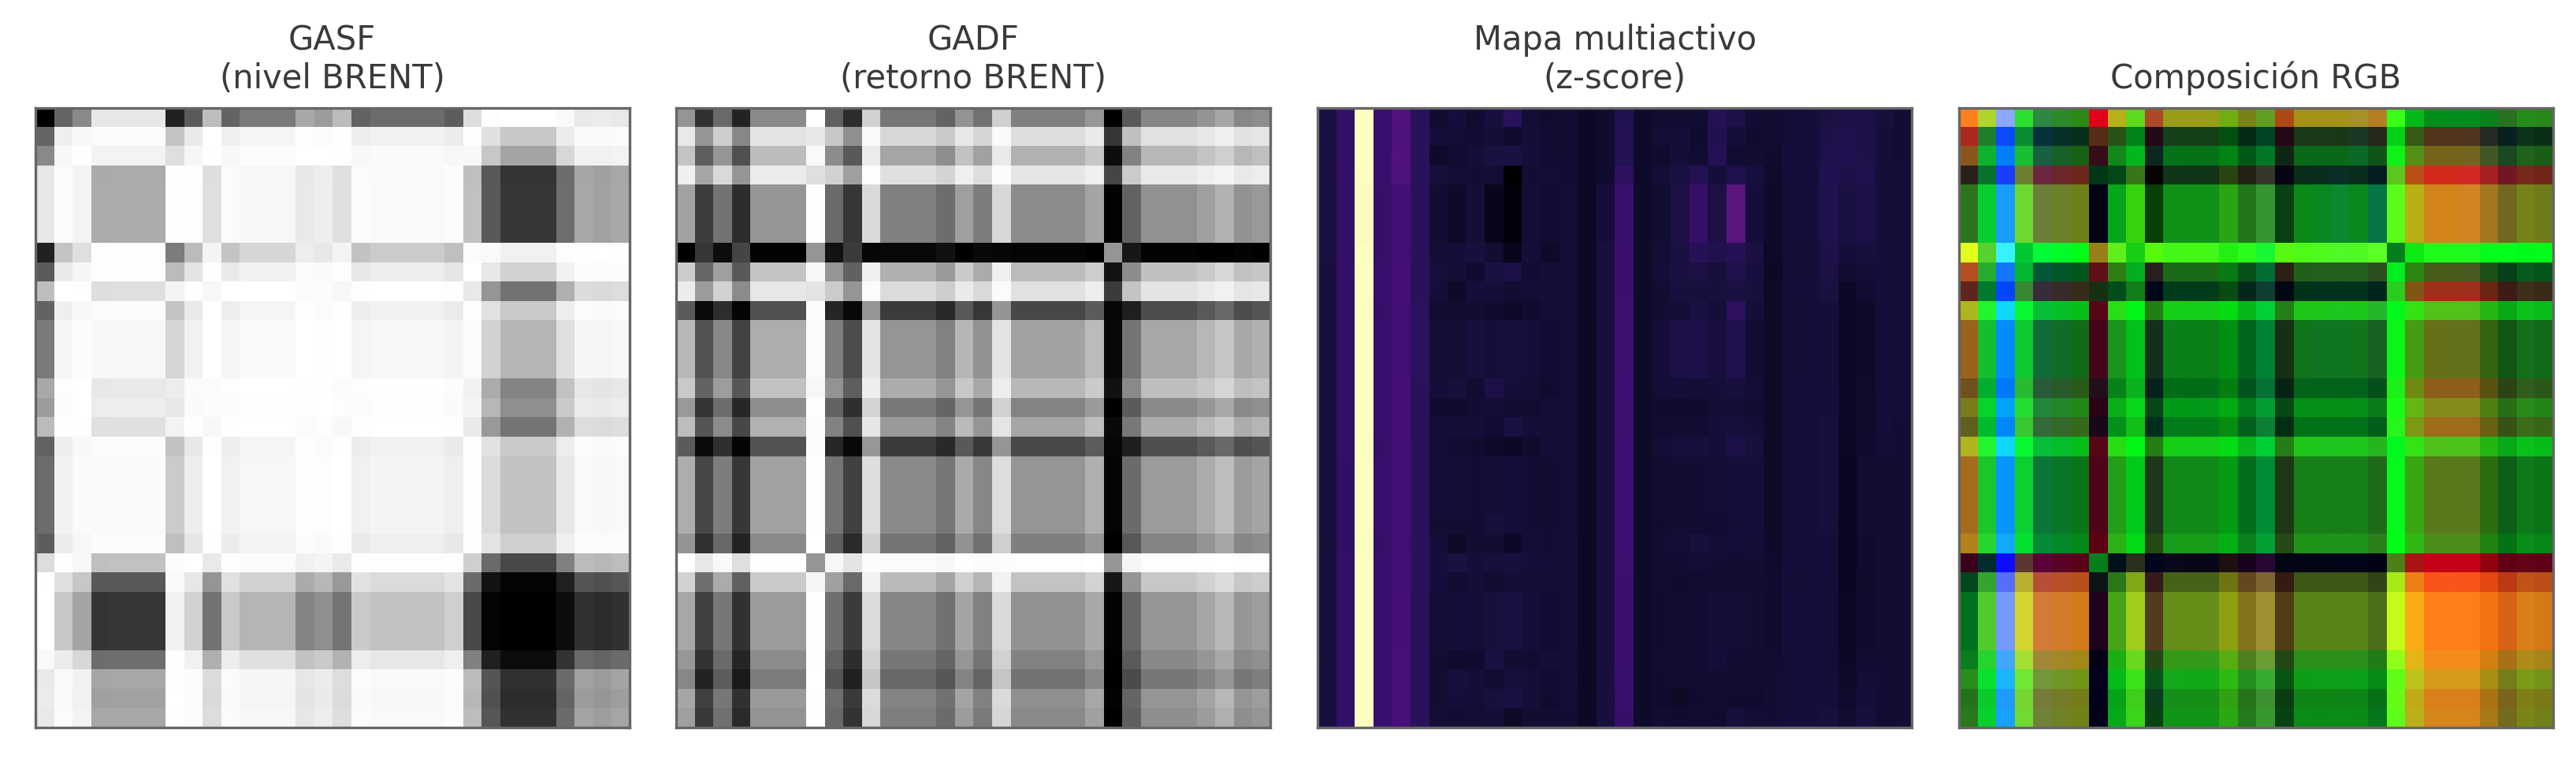
\includegraphics[width=0.95\textwidth]{rgb_channels_example.png}
    \caption{Canales de la representación RGB para una ventana real del BRENT.}
    \label{fig:rgbexample}
\end{figure}

\begin{figure}[H]
    \centering
    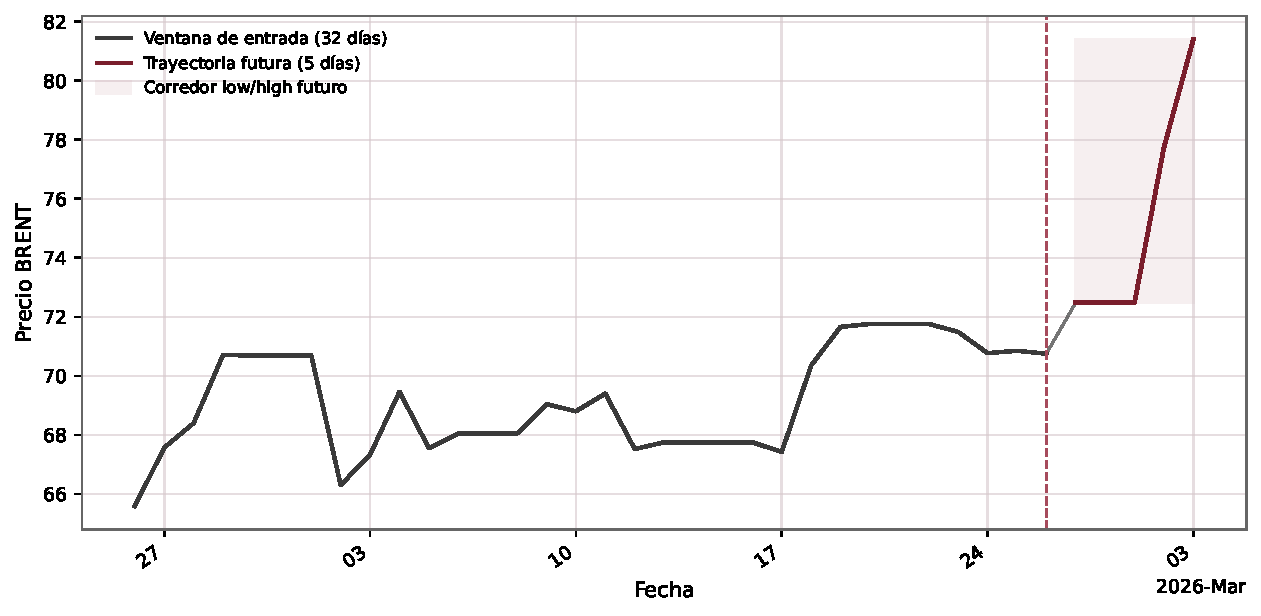
\includegraphics[width=0.86\textwidth]{example_window_future.pdf}
    \caption{Ventana de entrada de 32 días y corredor futuro de cinco días para una observación del tramo de test.}
    \label{fig:examplewindow}
\end{figure}

\section{Ecuaciones de la codificación GASF/GADF y de la CNN multitarea}

En la configuración analizada del proyecto, cada muestra parte de una ventana temporal de longitud $L=32$ y de una matriz multivariante con $F=180$ variables, que posteriormente se transforma en una imagen RGB de tamaño $160\times 160$. La salida del modelo combina clasificación de patrón y regresión de tres magnitudes continuas: \texttt{future\_return}, \texttt{future\_low} y \texttt{future\_high}.\footnote{Si en otra corrida cambia el conjunto de variables seleccionadas, basta con sustituir $F=180$ por el número efectivo de \emph{features}.}

\subsection{Ventana de entrada}

Sea
\begin{equation}
\mathbf{W}^{(n)} \in \mathbb{R}^{L \times F},
\qquad L=32,
\qquad F=180,
\end{equation}
la ventana $n$-ésima del bundle multivariante. Su fila $t$ contiene las $F$ variables observadas en el instante temporal $t$, y la serie objetivo de BRENT dentro de la ventana se denota por
\begin{equation}
\mathbf{b} = (b_1, b_2, \dots, b_L) \in \mathbb{R}^{L}.
\end{equation}

\subsection{Canal GASF del nivel de BRENT}

Primero se reescala la serie de niveles de BRENT al intervalo $[-1,1]$:
\begin{equation}
\tilde b_t = 2\,\frac{b_t - \min(\mathbf{b})}{\max(\mathbf{b}) - \min(\mathbf{b})} - 1,
\qquad t=1,\dots,L.
\end{equation}

Después se define la representación angular
\begin{equation}
\phi_t = \arccos(\tilde b_t),
\qquad \phi_t \in [0,\pi].
\end{equation}

El \emph{Gramian Angular Summation Field} se construye como
\begin{equation}
\mathrm{GASF}_{ij} = \cos(\phi_i + \phi_j),
\qquad i,j=1,\dots,L.
\end{equation}

Para su uso como canal de imagen, el mapa se normaliza a $[0,1]$:
\begin{equation}
\mathcal{N}(A) = \frac{A - \min(A)}{\max(A) - \min(A)}.
\end{equation}

Así, el canal rojo queda definido por
\begin{equation}
\mathbf{C}^{(R)} = \mathcal{R}_{160}\!\left(\mathcal{N}(\mathrm{GASF})\right),
\end{equation}
donde $\mathcal{R}_{160}(\cdot)$ representa el reescalado bidimensional a $160\times 160$.

\subsection{Canal GADF del retorno de BRENT}

La rama verde de la imagen se construye sobre el retorno discreto usado en la implementación:
\begin{equation}
 r_1 = 0,
 \qquad
 r_t = \frac{b_t - b_{t-1}}{\max(b_t,\varepsilon)},
 \qquad t=2,\dots,L,
\end{equation}
con $\varepsilon>0$ pequeño para evitar divisiones por cero.

Se reescala $\mathbf{r}=(r_1,\dots,r_L)$ a $[-1,1]$,
\begin{equation}
\tilde r_t = 2\,\frac{r_t - \min(\mathbf{r})}{\max(\mathbf{r}) - \min(\mathbf{r})} - 1,
\end{equation}
y se define
\begin{equation}
\psi_t = \arccos(\tilde r_t).
\end{equation}

El \emph{Gramian Angular Difference Field} viene dado por
\begin{equation}
\mathrm{GADF}_{ij} = \sin(\psi_i - \psi_j),
\qquad i,j=1,\dots,L.
\end{equation}

El canal verde es entonces
\begin{equation}
\mathbf{C}^{(G)} = \mathcal{R}_{160}\!\left(\mathcal{N}(\mathrm{GADF})\right).
\end{equation}

\subsection{Canal multivariante de \emph{features}}

La tercera capa codifica la matriz multivariante de \emph{features} de la ventana. Si
\begin{equation}
\mathbf{M} = \mathbf{W}^{\top} \in \mathbb{R}^{F \times L},
\end{equation}
entonces cada fila $\mathbf{m}_f$ representa la trayectoria temporal de la \emph{feature} $f$ dentro de la ventana.

La implementación aplica un escalado robusto por fila usando mediana e intervalo intercuartílico:
\begin{equation}
\widehat M_{f,t} = \frac{M_{f,t} - \operatorname{mediana}(\mathbf{m}_f)}{\operatorname{IQR}(\mathbf{m}_f)},
\qquad \operatorname{IQR}(\mathbf{m}_f)=Q_{0.75}(\mathbf{m}_f)-Q_{0.25}(\mathbf{m}_f).
\end{equation}

Después se comprime el rango a $[0,1]$ mediante saturación:
\begin{equation}
\overline M_{f,t} = \operatorname{clip}\!\left(\frac{\widehat M_{f,t}+3}{6},\,0,\,1\right).
\end{equation}

Finalmente, el canal azul se obtiene reescalando el mapa resultante a una matriz cuadrada:
\begin{equation}
\mathbf{C}^{(B)} = \mathcal{R}_{160}\!\left(\overline{\mathbf{M}}\right).
\end{equation}

\subsection{Composición de la imagen RGB}

La imagen final de entrada a la red se construye como
\begin{equation}
\mathbf{I} = 255\cdot \operatorname{stack}\left(\mathbf{C}^{(R)},\mathbf{C}^{(G)},\mathbf{C}^{(B)}\right)
\in [0,255]^{160\times 160\times 3}.
\end{equation}

Antes de entrar en el backbone, la imagen se normaliza con las estadísticas de ImageNet:
\begin{equation}
X_{cij} = \frac{I_{cij}/255 - \mu_c}{\sigma_c},
\qquad
\boldsymbol{\mu}=(0.485,0.456,0.406),
\quad
\boldsymbol{\sigma}=(0.229,0.224,0.225).
\end{equation}

\subsection{CNN multitarea con backbone EfficientNet-B1}

Sea
\begin{equation}
\mathbf{h} = f_{\mathrm{EffB1}}(\mathbf{X}) \in \mathbb{R}^{d}
\end{equation}
el vector latente devuelto por el backbone \textit{EfficientNet-B1} tras el \emph{global average pooling}. En la implementación del proyecto, este backbone se usa como extractor de características y se conecta a una cabeza compartida:
\begin{equation}
\mathbf{s} = \operatorname{Dropout}\!\left(\operatorname{SiLU}(\mathbf{W}_h\,\operatorname{Dropout}(\mathbf{h}) + \mathbf{b}_h)\right),
\qquad \mathbf{s}\in\mathbb{R}^{256}.
\end{equation}

La activación SiLU viene dada por
\begin{equation}
\operatorname{SiLU}(x)=x\,\sigma(x)=\frac{x}{1+e^{-x}}.
\end{equation}

A partir de la representación compartida, la cabeza de clasificación genera los logits
\begin{equation}
\mathbf{z}=\mathbf{W}_c\mathbf{s}+\mathbf{b}_c,
\qquad \mathbf{z}\in\mathbb{R}^{K},
\end{equation}
donde $K$ es el número de patrones chartistas. Las probabilidades se obtienen con \emph{softmax}:
\begin{equation}
 p_k = \frac{e^{z_k}}{\sum_{j=1}^{K}e^{z_j}},
 \qquad k=1,\dots,K.
\end{equation}

La cabeza de regresión produce simultáneamente tres salidas continuas:
\begin{equation}
\widehat{\mathbf{y}}^{\mathrm{reg}} = \mathbf{W}_r\mathbf{s}+\mathbf{b}_r
=\begin{bmatrix}
\widehat y_{\mathrm{return}} \\
\widehat y_{\mathrm{low}} \\
\widehat y_{\mathrm{high}}
\end{bmatrix}
\in \mathbb{R}^{3}.
\end{equation}

\subsection{Ecuación general de una capa convolucional}

Si se desea incluir la forma general de la operación convolucional que subyace al backbone, puede expresarse como
\begin{equation}
Y^{(\ell)}_{c_o,i,j} = b^{(\ell)}_{c_o} +
\sum_{c_i=1}^{C_{\mathrm{in}}}
\sum_{u=0}^{k_h-1}
\sum_{v=0}^{k_w-1}
W^{(\ell)}_{c_o,c_i,u,v}\,X^{(\ell-1)}_{c_i,\,i+u,\,j+v}.
\end{equation}

Tras la convolución, una forma compacta de la transformación no lineal es
\begin{equation}
\mathbf{A}^{(\ell)} = \operatorname{SiLU}\!\left(\operatorname{BN}\!\left(\mathbf{Y}^{(\ell)}\right)\right),
\end{equation}
y el \emph{global average pooling} final del backbone puede escribirse como
\begin{equation}
 h_c = \frac{1}{HW}\sum_{i=1}^{H}\sum_{j=1}^{W} A_{cij}^{(L_b)},
\end{equation}
donde $L_b$ denota la última capa convolucional del backbone.

\subsection{Función objetivo multitarea}

La pérdida total del modelo es la suma de una pérdida de clasificación y una pérdida de regresión ponderada:
\begin{equation}
\mathcal{L} = \mathcal{L}_{\mathrm{cls}} + \lambda\,\mathcal{L}_{\mathrm{reg}},
\qquad \lambda = 0.5.
\end{equation}

Para la clasificación se usa entropía cruzada:
\begin{equation}
\mathcal{L}_{\mathrm{cls}} = -\sum_{k=1}^{K} y_k\log p_k.
\end{equation}

En la rama PyTorch del proyecto, la pérdida de regresión es \emph{SmoothL1} sobre las tres salidas:
\begin{equation}
\mathcal{L}_{\mathrm{reg}} = \frac{1}{3}\sum_{m=1}^{3} \operatorname{SmoothL1}\!\left(\widehat y_m - y_m\right),
\end{equation}
con
\begin{equation}
\operatorname{SmoothL1}(u)=
\begin{cases}
\tfrac{1}{2}u^2, & \text{si } |u|<1,\\[4pt]
|u|-\tfrac{1}{2}, & \text{si } |u|\ge 1.
\end{cases}
\end{equation}

Si se documenta también la rama TensorFlow del mismo proyecto, la formulación es análoga pero sustituyendo \emph{SmoothL1} por pérdida de Huber.

\subsection{Modelo y flujo de procesamiento}
La propuesta del proyecto utiliza EfficientNet-B1 como extractor principal sobre la imagen RGB. A partir de la representación latente, una cabeza multitarea produce la distribución de probabilidad sobre patrones y las tres salidas continuas mencionadas. La función objetivo combina una pérdida de clasificación y una pérdida de regresión con peso relativo $\lambda = 0.5$:
\begin{equation}
\mathcal{L} = \mathcal{L}_{\mathrm{cls}} + \lambda\,\mathcal{L}_{\mathrm{reg}}.
\end{equation}

La Figura~\ref{fig:pipeline} resume los pasos metodológicos del estudio desde la descarga de series hasta la generación de reportes.

\begin{figure}[H]
    \centering
    
\includegraphics[width=0.94\textwidth]{pipeline_diagram.pdf}
    \caption{Resumen del flujo metodológico del experimento.}
    \label{fig:pipeline}
\end{figure}

\section{Resultados}
\subsection{Cobertura temporal y distribución de clases}
La Figura~\ref{fig:timeline} sitúa los tramos temporales de train, validación, test y última señal sobre la serie histórica del BRENT. El tramo etiquetado de evaluación comienza el 2 de diciembre de 2019 y el último punto con corredor futuro completo corresponde al 26 de febrero de 2026.

\begin{figure}[H]
    \centering
    
\includegraphics[width=0.92\textwidth]{brent_timeline.pdf}
    \caption{Trayectoria del BRENT y localización temporal de las particiones evaluadas.}
    \label{fig:timeline}
\end{figure}

La distribución de etiquetas débiles es marcadamente desbalanceada. Predominan \texttt{ascending\_channel}, \texttt{descending\_channel} y \texttt{range}, mientras que \texttt{high\_tight\_flag} y \texttt{head\_shoulders} no aparecen en la muestra evaluada. La Figura~\ref{fig:labels} y la Tabla~\ref{tab:classsupport} resumen esta estructura.

\begin{figure}[H]
    \centering
    
\includegraphics[width=0.80\textwidth]{weak_label_distribution.pdf}
    \caption{Distribución de etiquetas débiles en las ventanas supervisadas.}
    \label{fig:labels}
\end{figure}

\begin{table}[H]
\centering
\footnotesize
\caption{Soporte por patrón en las ventanas evaluadas y número de predicciones emitidas sobre esas mismas fechas.}
\label{tab:classsupport}
\begin{adjustbox}{max width=0.84\textwidth}
\begin{tabular}{lrr}
\toprule
                Patrón &  Ventanas etiquetadas &  Predicciones en las mismas fechas \\
\midrule
     ascending\_channel &                   506 &                                633 \\
    descending\_channel &                   418 &                                451 \\
                 range &                   248 &                                133 \\
            double\_top &                    37 &                                  7 \\
         double\_bottom &                    20 &                                  3 \\
inverse\_head\_shoulders &                     1 &                                  1 \\
\bottomrule
\end{tabular}

\end{adjustbox}
\end{table}

\subsection{Resultados de clasificación y regresión}
La Tabla~\ref{tab:metrics} presenta el rendimiento agregado por partición. En test, la exactitud frente a etiquetas débiles es 53.3\%, la exactitud top-2 asciende al 81.6\% y la MAE del retorno a un día es 2.64 puntos porcentuales. La diferencia entre train y validación/test sugiere un ajuste insuficiente del modelo bajo el régimen corto de entrenamiento empleado en esta corrida.

\begin{table}[H]
\centering
\footnotesize
\caption{Métricas agregadas por partición.}
\label{tab:metrics}
\begin{adjustbox}{max width=\textwidth}
\begin{tabular}{lrrrrrrrrr}
\toprule
Partición &    n & Exactitud (\%) & Top-2 (\%) & MAE retorno (pp) & RMSE retorno (pp) & Acierto signo (\%) &    R2 & MAE low (pp) & MAE high (pp) \\
\midrule
    train &  887 &          85.0 &      95.3 &             3.15 &              4.11 &             52.20 & -1.27 &         4.17 &          3.88 \\
    valid &   99 &          53.5 &      77.8 &             3.17 &              3.94 &             47.47 & -4.59 &         3.58 &          3.26 \\
     test &  244 &          53.3 &      81.6 &             2.64 &              3.40 &             52.46 & -2.43 &         3.51 &          3.72 \\
      all & 1230 &          76.2 &      91.1 &             3.05 &              3.97 &             51.87 & -1.51 &         3.99 &          3.80 \\
\bottomrule
\end{tabular}

\end{adjustbox}
\end{table}

La Figura~\ref{fig:confusion} muestra la matriz de confusión normalizada en test y la Tabla~\ref{tab:testclass} detalla precisión, recall y F1 para las clases presentes en ese tramo. Los resultados indican una mejor separación relativa de \texttt{ascending\_channel} y \texttt{descending\_channel}, mientras que \texttt{range} presenta una recuperación mucho más limitada.

\begin{figure}[H]
    \centering
    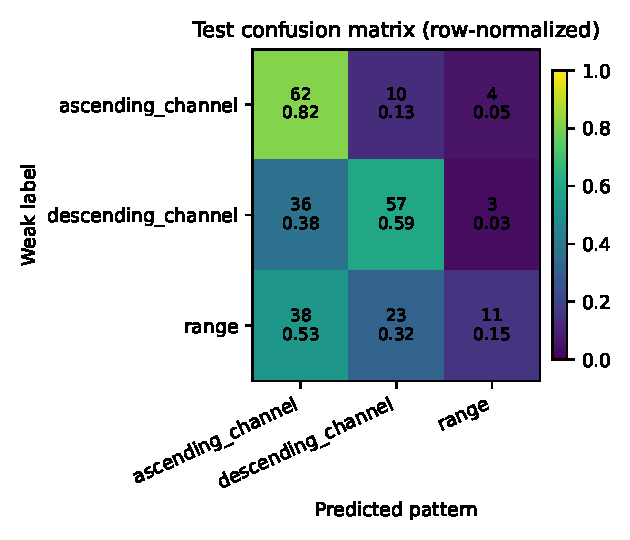
\includegraphics[width=0.56\textwidth]{test_confusion_matrix.pdf}
    \caption{Matriz de confusión normalizada por filas en el conjunto de test.}
    \label{fig:confusion}
\end{figure}

\begin{table}[H]
\centering
\footnotesize
\caption{Informe de clasificación en test.}
\label{tab:testclass}
\begin{adjustbox}{max width=0.72\textwidth}
\begin{tabular}{lrrrr}
\toprule
             Clase & Precision (\%) & Recall (\%) & F1 (\%) & Soporte \\
\midrule
 ascending\_channel &          45.6 &       81.6 &   58.5 &      76 \\
descending\_channel &          63.3 &       59.4 &   61.3 &      96 \\
             range &          61.1 &       15.3 &   24.4 &      72 \\
          accuracy &             — &          — &   53.3 &     244 \\
\bottomrule
\end{tabular}

\end{adjustbox}
\end{table}

La serie temporal de predicciones de retorno, representada en la Figura~\ref{fig:testreturns}, muestra que el modelo capta parcialmente episodios de dirección correcta, pero la magnitud de los movimientos sigue siendo difícil de aproximar de forma estable.

\begin{figure}[H]
    \centering
    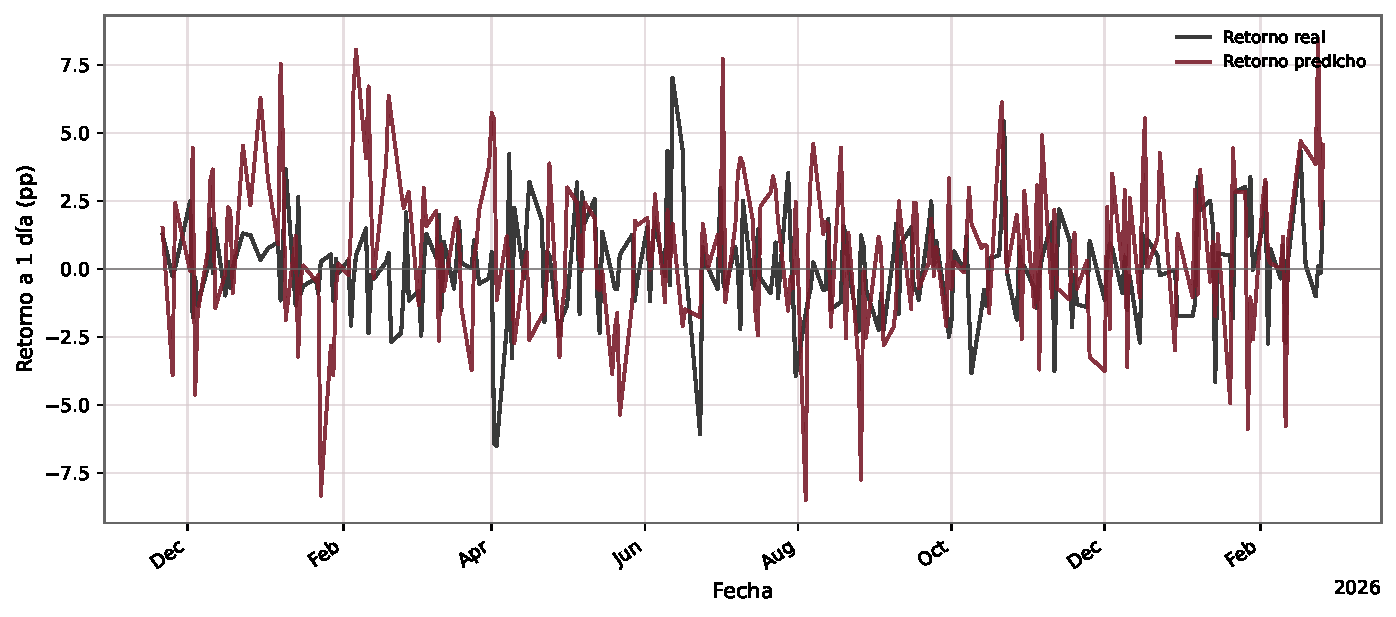
\includegraphics[width=0.92\textwidth]{test_return_timeseries.pdf}
    \caption{Retorno real frente a retorno predicho sobre el tramo de test.}
    \label{fig:testreturns}
\end{figure}

\subsection{Última señal y análisis de outliers}
La última señal disponible corresponde al 6 de marzo de 2026. La Tabla~\ref{tab:latest} resume sus valores principales y la Figura~\ref{fig:latestprob} representa la distribución de probabilidad por patrón.

\begin{table}[H]
\centering
\footnotesize
\caption{Última señal disponible del sistema.}
\label{tab:latest}
\begin{adjustbox}{max width=0.72\textwidth}
\begin{tabular}{p{0.45\textwidth}p{0.22\textwidth}}
\toprule
                            Campo &             Valor \\
\midrule
                Fecha de la señal &        2026-03-06 \\
                 Patrón dominante & ascending\_channel \\
                    Precio actual &             85.41 \\
             Retorno esperado (\%) &             0.987 \\
                     Pred low (\%) &             0.455 \\
                    Pred high (\%) &            -2.992 \\
                   Nivel objetivo &            86.253 \\
                 Nivel de soporte &            85.798 \\
             Nivel de resistencia &            82.854 \\
Confianza dominante en la ventana &             0.400 \\
           Weighted outlier score &             0.496 \\
                     Outlier flag &                 1 \\
\bottomrule
\end{tabular}

\end{adjustbox}
\end{table}

\begin{figure}[H]
    \centering
    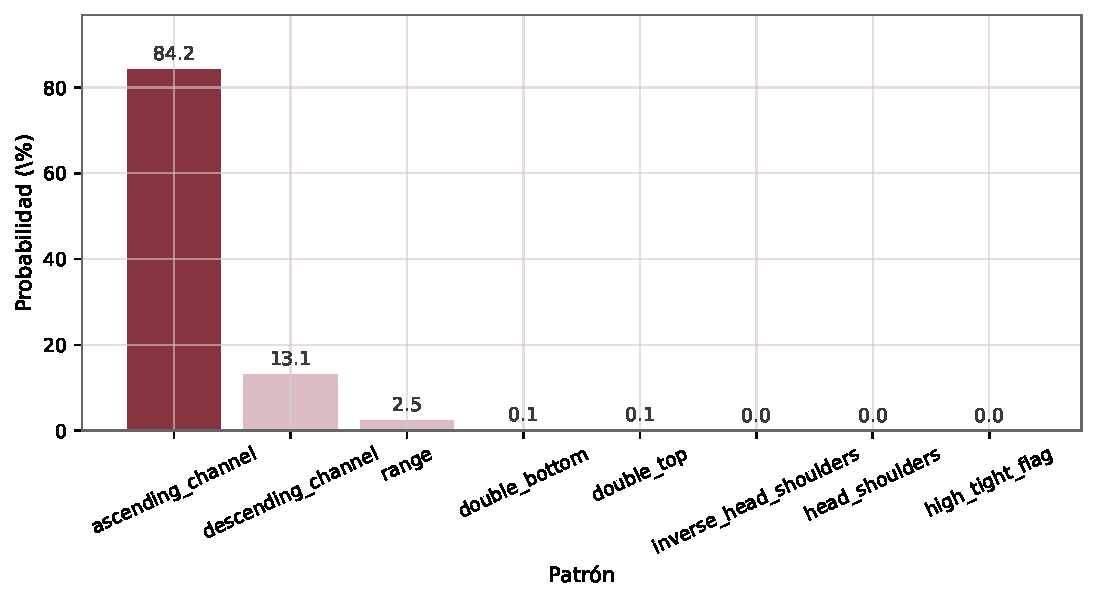
\includegraphics[width=0.86\textwidth]{latest_signal_probabilities.pdf}
    \caption{Probabilidades por patrón para la última señal disponible.}
    \label{fig:latestprob}
\end{figure}

En esta observación, el patrón dominante es \texttt{ascending\_channel} con probabilidad 0.842. El retorno esperado a un día es positivo, pero la pareja \texttt{pred\_low/pred\_high} queda invertida respecto a los niveles de soporte y resistencia. Dado que ambas salidas se estiman de forma independiente, esta inversión debe interpretarse como una limitación del esquema de regresión y no como una inconsistencia de transcripción.

El sistema marca 942 observaciones como outliers dentro de 2290 ventanas inferidas, lo que equivale al 41.1\%. La Figura~\ref{fig:outliers} muestra que esta activación se debe casi por completo a baja confianza dominante y sólo de forma residual a distancia métrica elevada; el umbral principal del \emph{weighted score} no llega a activarse en la corrida aportada.

\begin{figure}[H]
    \centering
    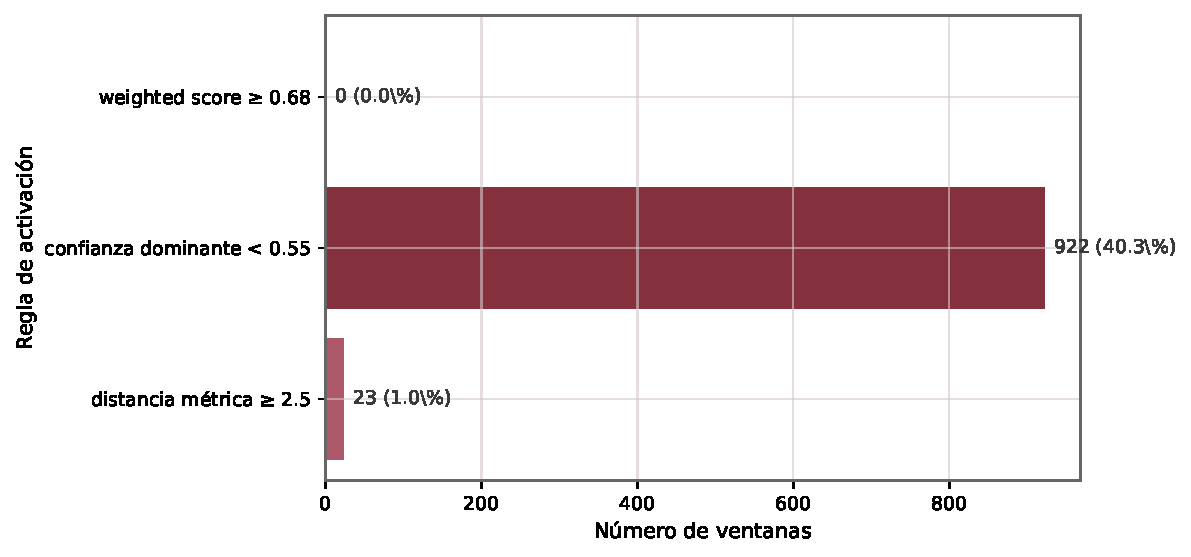
\includegraphics[width=0.88\textwidth]{outlier_triggers.pdf}
    \caption{Descomposición de las reglas que activan la bandera de outlier.}
    \label{fig:outliers}
\end{figure}
\newpage
\section{Discusión}
Los resultados empíricos muestran que la codificación RGB conserva información suficiente para discriminar patrones dominantes sobre BRENT cuando se combina con contexto multiactivo. Sin embargo, la calidad de la discriminación depende de forma importante del desbalance entre clases y del régimen de entrenamiento. La mejora notable en train frente a validación y test sugiere que esta corrida debe leerse como una validación funcional del pipeline, más que como una estimación final del rendimiento del método.

También hay restricciones propias de los datos. La ausencia de los cuatro nodos AAA del BCE previstos en el descargador reduce el universo macro-financiero originalmente planteado. Además, la disponibilidad tardía de \texttt{ESTR} y \texttt{SOFR} comprime la muestra útil con todas las variables presentes. Desde el punto de vista de la salida continua, la inversión ocasional entre \texttt{pred\_low} y \texttt{pred\_high} sugiere que una versión posterior del sistema debería imponer restricciones de orden o una parametrización coherente para dichos niveles.

\section{Conclusiones}
El experimento confirma que un esquema basado en ventanas multiactivo, codificación RGB y EfficientNet-B1 puede aplicarse al reconocimiento automático de patrones chartistas sobre BRENT en un marco multitarea. Con 180 variables de entrada y ventanas de 32 observaciones, la corrida analizada alcanza 53.3\% de exactitud y 81.6\% de top-2 en test, junto con una MAE de 2.64 puntos porcentuales para el retorno a un día.

Desde una perspectiva metodológica, el principal valor del estudio es que explicita el vínculo entre fuentes de mercado heterogéneas, representación visual de la ventana y salida conjunta de clasificación y regresión. Como líneas de continuación, resultan especialmente relevantes un régimen de entrenamiento más largo, estrategias de balanceo entre clases, la recuperación de las series del BCE inicialmente previstas y la incorporación de restricciones estructurales sobre las salidas continuas de niveles futuros.

\begin{thebibliography}{9}

\bibitem{tan2019efficientnet}
Mingxing Tan and Quoc V. Le.
\newblock EfficientNet: Rethinking Model Scaling for Convolutional Neural Networks.
\newblock In \emph{Proceedings of the 36th International Conference on Machine Learning}, pages 6105--6114, 2019.

\bibitem{wang2015imaging}
Zhiguang Wang and Tim Oates.
\newblock Imaging Time-Series to Improve Classification and Imputation.
\newblock In \emph{Proceedings of the 24th International Joint Conference on Artificial Intelligence}, pages 3939--3945, 2015.

\bibitem{lo2000foundations}
Andrew W. Lo, Harry Mamaysky, and Jiang Wang.
\newblock Foundations of Technical Analysis: Computational Algorithms, Statistical Inference, and Empirical Implementation.
\newblock \emph{The Journal of Finance}, 55(4):1705--1765, 2000.

\end{thebibliography}

\end{document}
